\documentclass[12pt]{article}

\usepackage{graphicx}
\usepackage{amsmath}
\usepackage{amssymb}
\usepackage{natbib}
\usepackage{amsfonts}
\usepackage{multicol}
\usepackage{float}
\usepackage{oldgerm}
\usepackage{bm}
\usepackage{mathtools}
\usepackage{wrapfig}
\usepackage{fancyhdr}
\usepackage[export]{adjustbox}
\usepackage{xcolor}
\usepackage[shortlabels]{enumitem}

\pagestyle{empty}

\setlength{\headsep}{0.5cm}
\setlength{\oddsidemargin}{-0.5cm}
\setlength{\textwidth}{16.5cm}
\setlength{\textheight}{24cm}
\voffset = -2cm


\pagestyle{fancy}
\fancyhf{}
\rfoot{
\includegraphics[width=1.0in]{cnm.png}}
\lfoot{Homework 4}
\setlength\parindent{0pt}
\begin{document}

\begin{center}
\hfil
{\large\bf {ENGR 2910-101: Circuit Analysis}}
\hfill Instructor: Brian Rashap\\
Homework 4 \hfill Due: See Brightspace\\
\hrulefill\\
\end{center}

{\bf Question 1} [4] % P4-6

Use the node-voltage method to find: $v_{o}$ and the power developed in the voltage source.

\begin{figure}[h!]
\begin{center}
 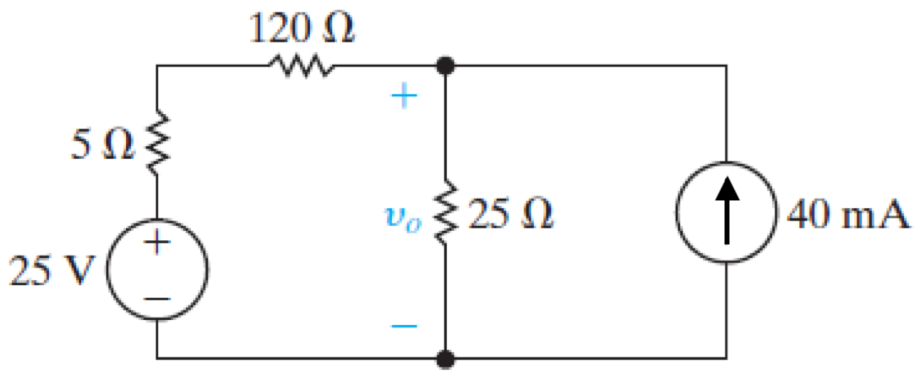
\includegraphics[clip,width=0.6\textwidth]{Fig4-6-v2.png}
\end{center}
\end{figure}


\vspace{0.1in}

{\bf Question 2} [4] %P4-11

Use the node-voltage method to find $v_{1}$ and $v_{2}$ in the circuit below.
\begin{figure}[h!]
\begin{center}
 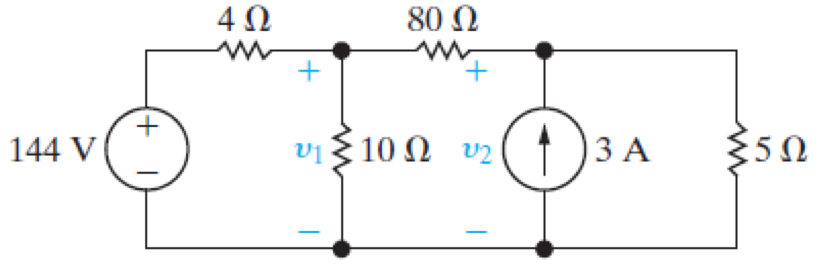
\includegraphics[clip,width=0.6\textwidth]{Fig4-11.png}
\end{center}
\end{figure}

{\bf Question 3} [4] %P4-15

Use the node-voltage method to find the voltages shown, $v_{1}$, $v_{2}$, and $v_{3}$.

\begin{figure}[h!]
\begin{center}
 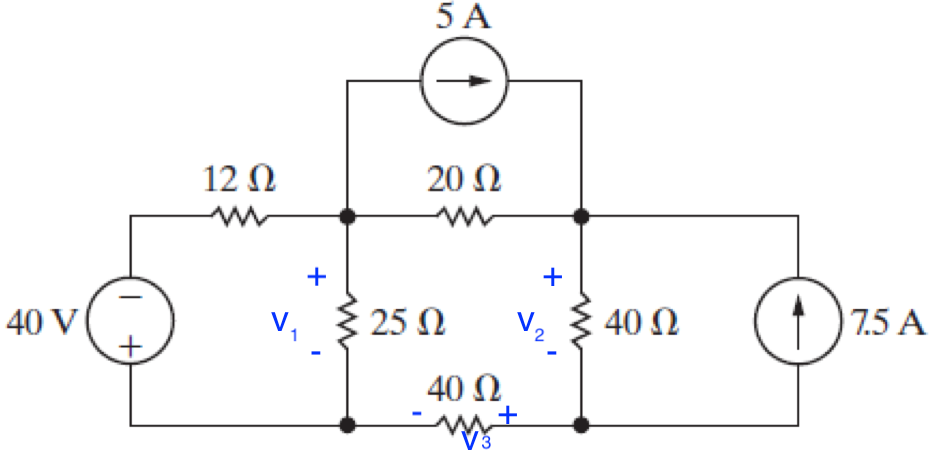
\includegraphics[clip,width=0.6\textwidth]{Fig4-15.png}
\end{center}
\end{figure}

\newpage
{\bf Question 4} [4] %P4-28

Use the node-voltage method to find $v_{o}$ in the circuit shown below.

\begin{figure}[h!]
\begin{center}
 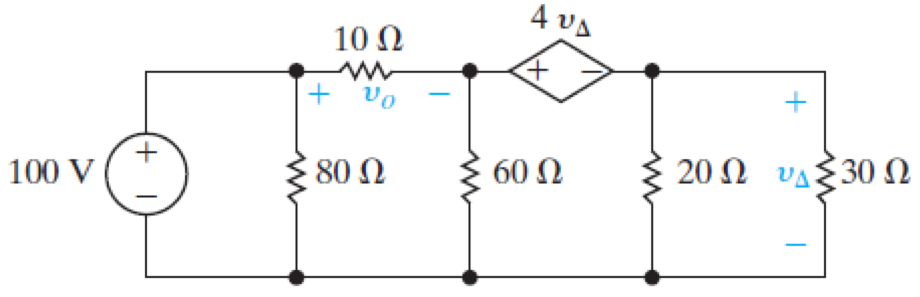
\includegraphics[clip,width=0.6\textwidth]{Fig4-28.png}
\end{center}
\end{figure}

{\bf Question 5} [4] %P4-29

Use the node-voltage method to find: [Hints: identify the supernode and also use the node labeled {\color{red} a}.]

\begin{figure}[h!]
\begin{center}
 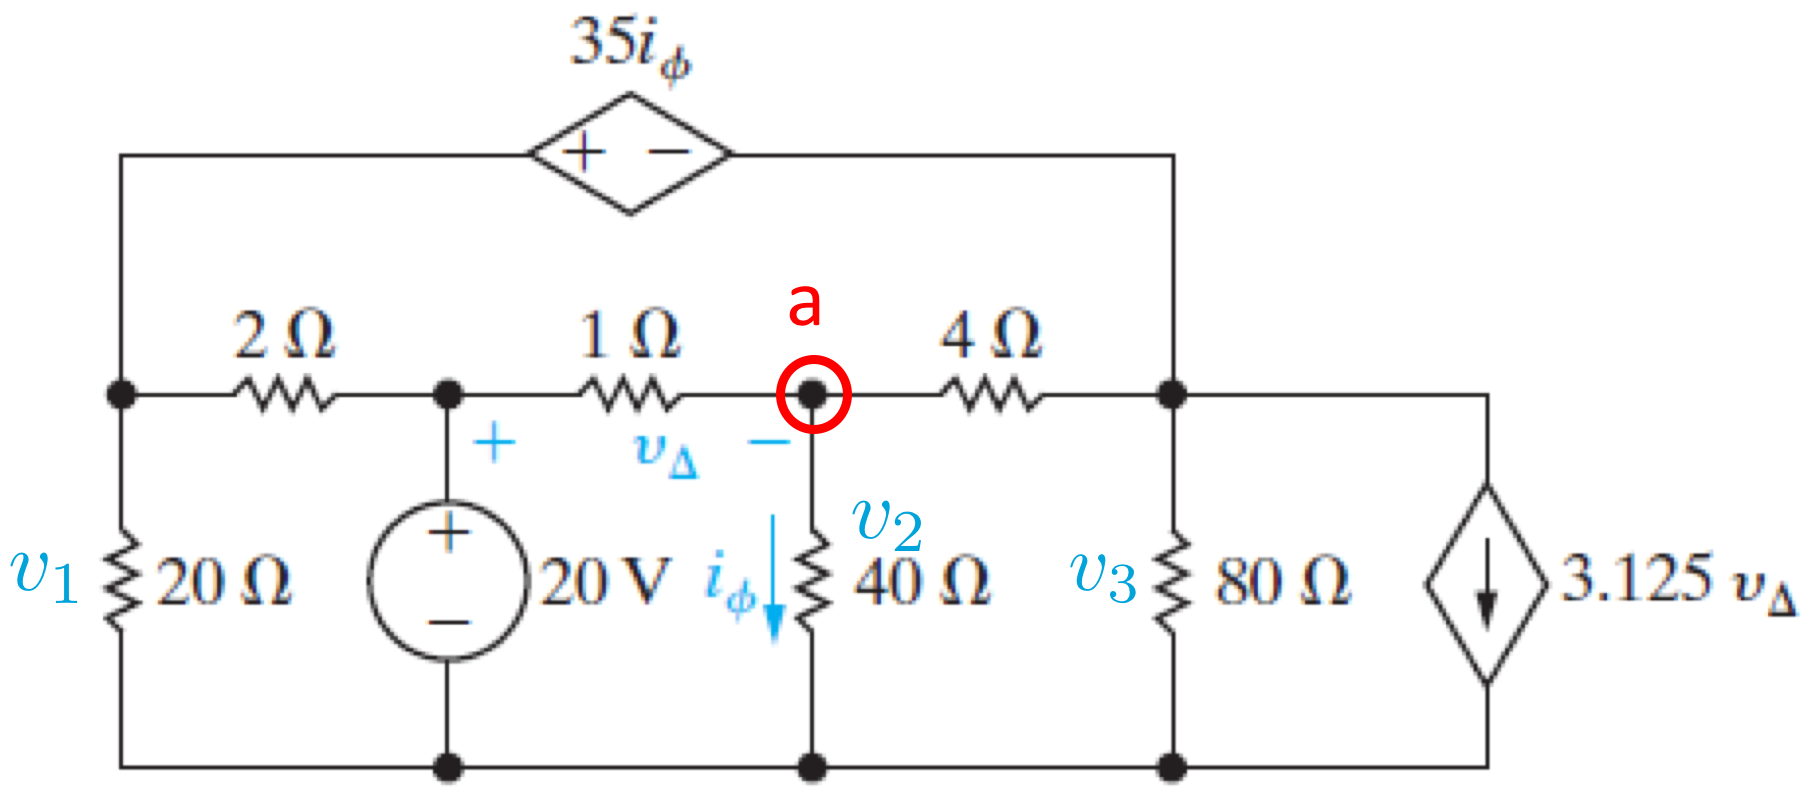
\includegraphics[clip,width=0.6\textwidth]{Fig4-29.png}
\end{center}
\end{figure}

\begin{enumerate}[(a)]
\item the voltage across the 20 $\Omega$ resistor, $v_{1}$, 
\item the voltage across the 40 $\Omega$ resistor, $v_{2}$, 
\item the voltage across the 80 $\Omega$ resistor, $v_{3}$, 
\item the controlling voltage, $v_{\Delta}$, 
\item the controlling current, $i_{\phi}$. 
\end{enumerate}
 
\end{document}
